\chapter{Identify ambiguous tasks}
\enlargethispage{3\baselineskip}

\begin{keypointstwomargins}{Identify ambiguous tasks}{-2cm}{-1cm}

        \textbf{Key points -- Identify ambiguous tasks}
        \begin{enumerate}[leftmargin=*]
        \item We know that datasets with better quality will lead to better models. It is famously a complicated task to explore big datasets and find ambiguous tasks in a classical supervised setting. What can we do for crowdsourced datasets?
        \item While entropy or variance-based methods in distribution votes are useful to retrieve tasks that lead to very noisy decisions, they are not fit in settings with few votes per task. And even less fitted to settings where a task can be labeled by a single worker. Can we still exploit these tasks?
        \end{enumerate}

        \textbf{Contributions -- Weighted Area Under the Margin}
        \begin{enumerate}[leftmargin=*,start=3]
        \item Following the literature on label noise, we adapt the AUM by \citet{pleiss_identifying_2020} into the AUMC and WAUM, two strategies to identify ambiguous tasks in datasets. The first is the baseline and directly falls back to the classical AUM using a majority vote. The WAUM introduces a trust score in the balance not to use poorly performing workers' answers.
        \item We provide a simple guideline: pruning most ambiguous tasks from the dataset, and reporting computer vision classifier performance with and without pruning on simulated and three real datasets: \texttt{CIFAR-10H}, \texttt{LabelMe} and \texttt{Music}.
        \end{enumerate}

\end{keypointstwomargins}

\section{Do we know what is in our training sets?}
While our datasets are getting larger and larger every year, one question naturally arises: \emph{What is the quality of our training sets?}
Indeed, small datasets can easily be looked at, but thousands of images -- if not millions -- represent herculean human work without assistance.
Mistakes happen, and the quality of the data is not always perfect (\Cref{fig:label_mistakes}).

\begin{figure}[thb]
\centering
\begin{minipage}{.3\linewidth}
\centering
\subfloat[$y^\star=\texttt{cat}$ in CIFAR-10 \citep{krizhevsky2009learning}]{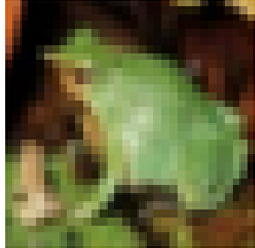
\includegraphics[width=\textwidth]{./chapters/images/catcifar.pdf}}
\end{minipage}%
\hfill
\begin{minipage}{.3\linewidth}
\centering
\subfloat[$y^\star=\texttt{tshirt}$ in Quickdraw]{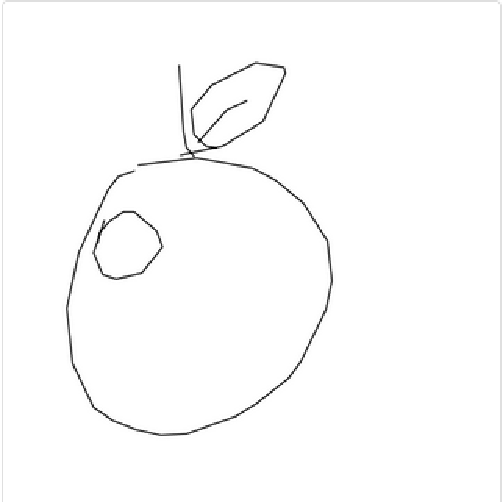
\includegraphics[width=\textwidth]{./chapters/images/tshirtquickdraw.pdf}}
\end{minipage}%
\hfill
\begin{minipage}{.3\linewidth}
\centering
\subfloat[$y^\star=\texttt{6}$ in MNIST \citep{deng2012mnist}]{
\includegraphics[width=\textwidth]{./chapters/images/6mnist.pdf}}
\end{minipage}
\caption{Three examples of labeling mistakes in classical classification datasets. The label can be wrong (CIFAR-10 and Quickdraw) or the task can be too ambiguous to classify (MNIST).}
\label{fig:label_mistakes}
\end{figure}


Data quality is linked with model performance \citep{budach2022effects}, looking for outliers to prune or weight differently during the learning procedure is not new \citep{angelova2004data}.
In this chapter, we first present the Area Under the Margin ($\AUM$): a statistic from \citet{pleiss_identifying_2020} that uses model iterates score prediction to detect unreliable training data points in the classically supervised learning setting.
Then, we propose to extend the $\AUM$ to the crowdsourcing setting with the Weighted Areas Under the Margin ($\WAUM$).
We show that the $\WAUM$ allows the identification of ambiguous tasks in crowdsourced datasets, and pruning a portion of those tasks leads to better test performance overall.

\subsection{Detect labeling errors in classical datasets}
% Cleanlab, confident learning, aum (litterature presentation and motivation mostly)
In classically supervised learning settings, training sets, tasks are paired up with a single label: $\mathcal{D}_\text{train}:=\{(x_i,y_i)\}_{i\in [n_\text{task}]}$.
This label has been assigned either automatically or via human decision.
Thus, the task might be mislabeled.
We can see a mislabeled task as a task that is difficult to classify for the classifier given this wrong label.
The $\AUM$ from \citet{pleiss_identifying_2020} allows us to identify tasks that are the most difficult to classify from the dataset.

More formally, the $\AUM$ of a task $(x_i,y_i)$ from a training set $\mathcal{D}_\text{train}$ given a classifier $\mathcal{C}$ and a number of training epochs $T>0$ is defined as:
\begin{equation}\label{eq:aum}
    \mathrm{AUM}\left(x, y; \mathcal{D}_{\texttt{train}}\right)
    = \!\! \frac{1}{T}\sum_{t=1}^T \!\! \big[\sigma^{(t)}_{y} (x)- \sigma^{(t)}_{[2]}(x)\big]
    \enspace.
\end{equation}
The $\AUM$ averages over time how far the score for the given class is from the most predicted other class by the classifier.
This is an average over time of the prediction margin.
It is classic to look at this margin in the literature to bound test error.
For example, \citet{bartlett1998boosting} showed that test error is dependent on the margin's distribution over the training set, even with zero error reached during training.
However, the $\AUM$ does not consider the margin given a trained classifier but looks at the early dynamics in the training procedure.
\citet{pleiss_identifying_2020} use an average of margins over logit scores, while we rather consider the average of margin after a softmax step in \Cref{eq:aum},
% Indeed, the original $\mathrm{AUM}$ relies on logit scores by applying a $\softmax$ step.
to temper scaling issues, as advocated by \citet{ju2018relative} in ensemble learning.
Moreover, we consider the margin introduced by \citet{yang2020consistency} since the corresponding hinge loss has better theoretical properties than the one used in the original $\mathrm{AUM}$, especially in top-$k$ settings\footnote{For top-$k$, consider $\sigma^{(t)}_{[k+1]}(x)$ instead of $\sigma^{(t)}_{[2]}(x)$ in \eqref{eq:aum}.} \citep{lapin2016loss, yang2020consistency,Garcin_Servajean_Joly_Salmon22}. However, one could easily consider the original margin with few differences in practice for top-$1$ classification.

\begin{figure}[thb]
\begin{minipage}{.45\linewidth}
\centering
\subfloat[Mislabeled image: $\AUM\ll 0$]{\label{mnist:low}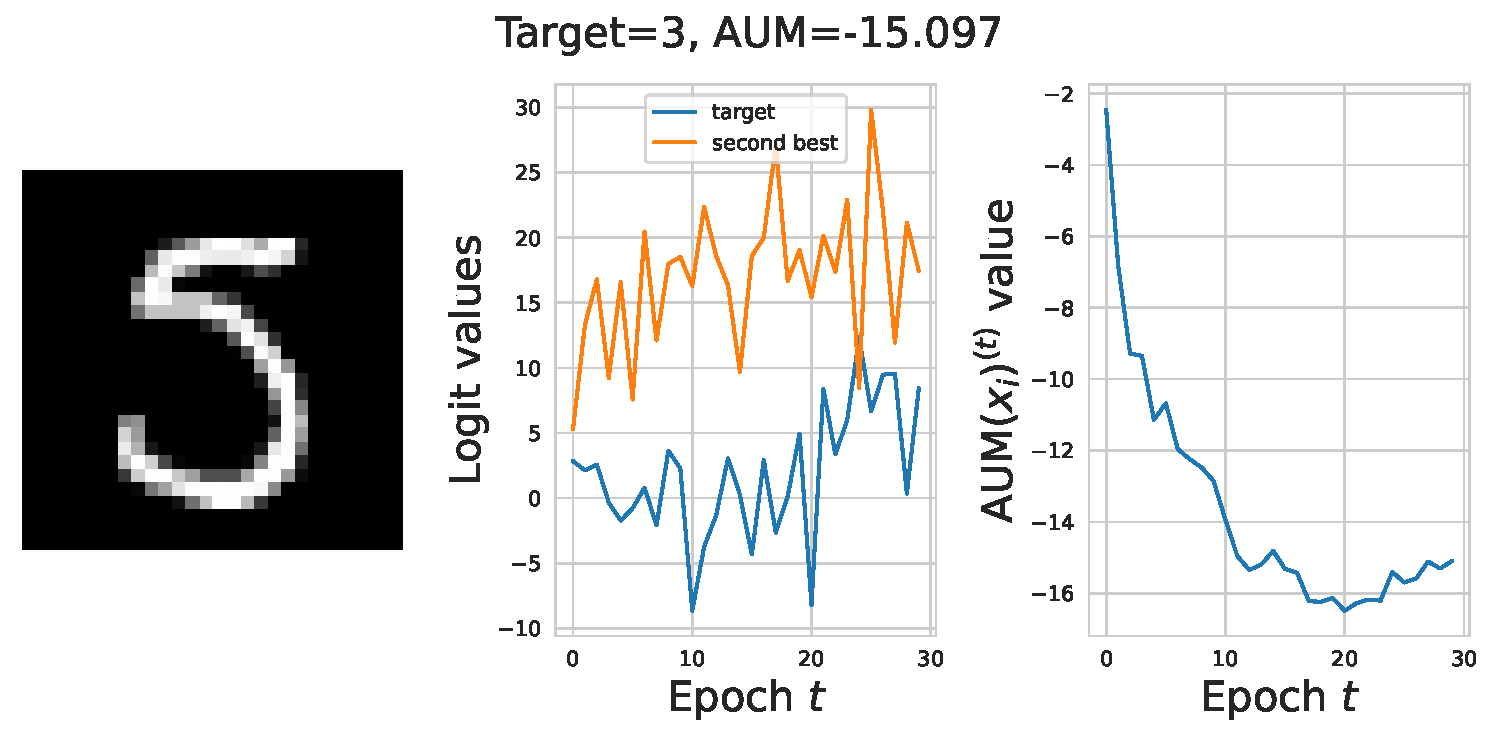
\includegraphics[width=\textwidth]{chapters/images/low_aum_mnist.pdf}}
\end{minipage}%
\hfill
\begin{minipage}{.45\linewidth}
\centering
\subfloat[Correct label: $\AUM\gg 0$]{\label{mnist:high}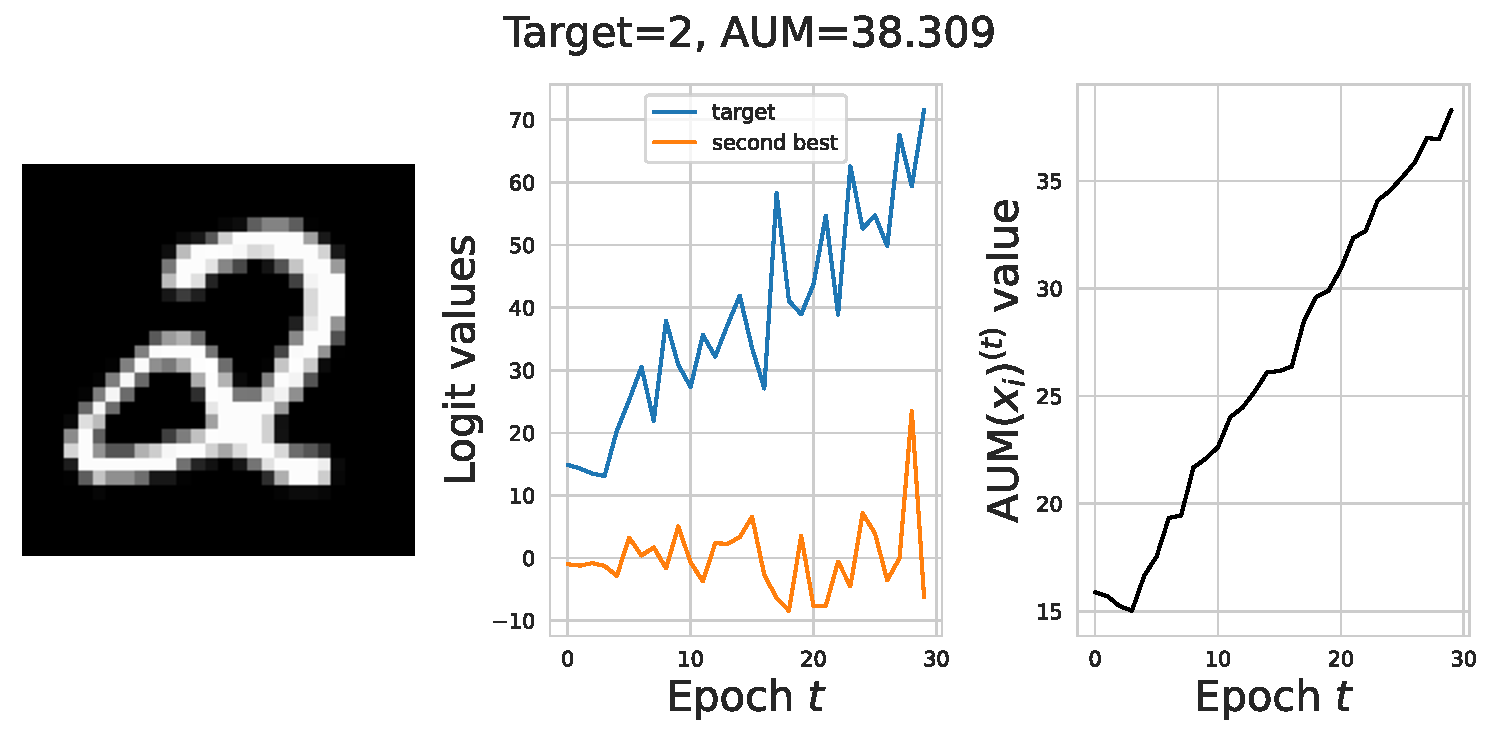
\includegraphics[width=\textwidth]{chapters/images/high_aum_mnist.pdf}}
\end{minipage}\par\medskip
\begin{center}
\subfloat[Confusion: the image is either a four or a nine cut-out with true label $y_i^\star=9$, the $\AUM$ is closer to zero indicating high ambiguity in learning classes]{\label{mnist:mid}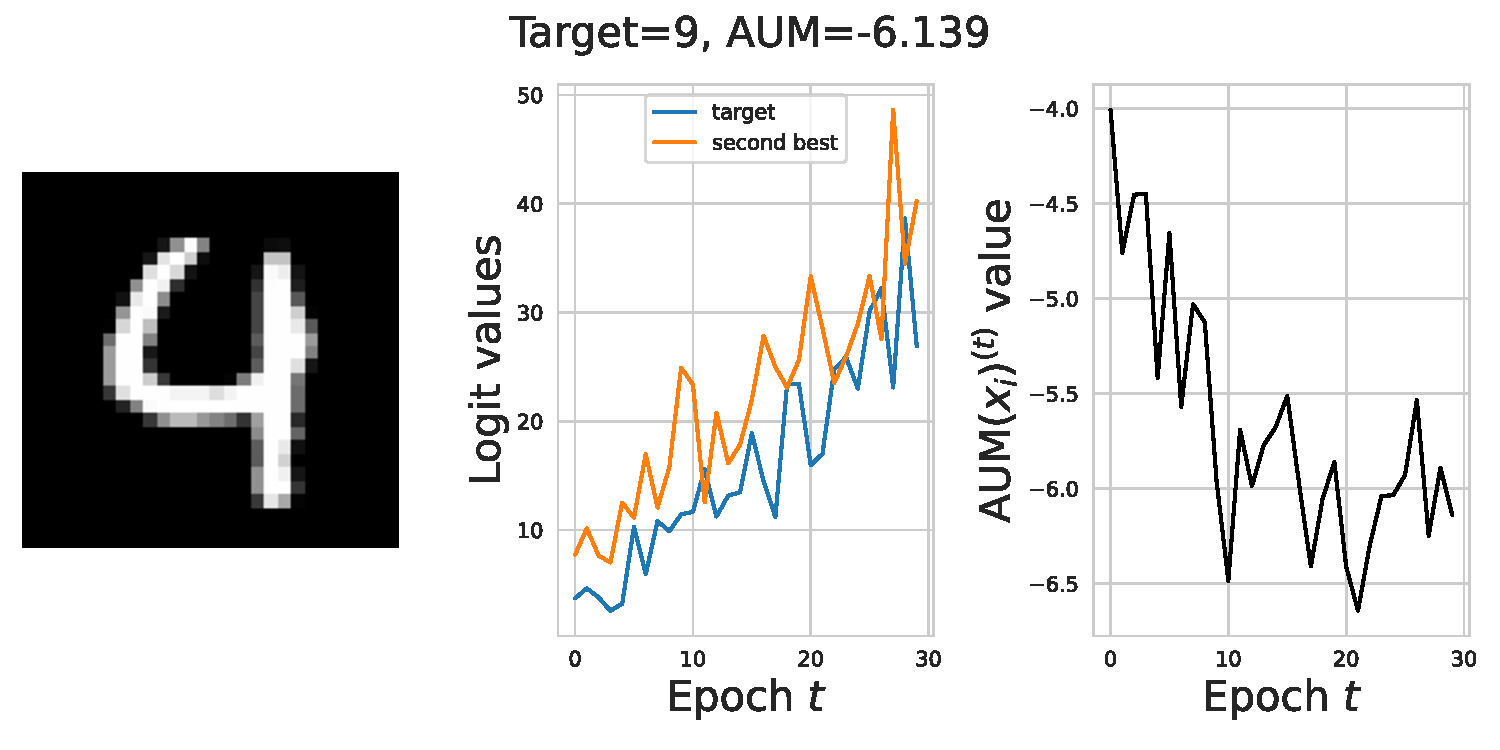
\includegraphics[width=.6\textwidth]{chapters/images/mid_aum_mnist.pdf}}
\end{center}
\caption{Three examples from the MNIST dataset to illustrate the behavior of the $\AUM$: if the sample is mislabeled the $\AUM$ is low as the classifier disagrees with the given label. Note that if $T>0$ is too high the memorization kicks in and the $\AUM$ increases again. When the sample is correctly labeled the $\AUM$ increases over training. When the sample is ambiguous, the $\AUM$ is closer to $0$. Results are from a 2-layer convolution network with max-pooling. Training is done in $T=30$ epochs using Adam optimizer with a learning rate set to $0.01$ and batches of $100$ samples.}
\label{fig:mnist_aum}
\end{figure}

This early dynamic, and by association with the hyperparameter $T>0$, is necessary as it is well known that modern neural networks classifiers can memorize the data and even classify correctly random tasks because of the hyperparametrization \citep{maennel2020neural}.
Memorization is a necessary phenomenon for training a neural network: we need the classifier to memorize patterns.
But what we wish to consider the least in the $\AUM$ is the unintended memorization \citep{maennel2020neural} that can happen early and is difficult to temper -- even with strategies like dropout or weight decay.
And in \citet{zhang2021understanding}, they show -- among other results -- that true labels are learned faster than random labels by neural networks classifier.
This early training dynamic in the prediction logits can thus be used as a proxy to identify possible mislabeled data.

Note that there exist other algorithms to learn from mislabeled data, such as Confident Learning \citep{northcutt_confident_2021} using by \texttt{CleanLab}\footnote{\url{https://cleanlab.ai/}}.
Confident Learning does not correct the label nor does it re-weight the data.
It estimates the joint distribution between the given and unknown latent labels with class-conditional noise and then prunes samples by class with a threshold of the average predicted probability for the samples in the given class.
With the $\AUM$, we can also correct the label during training -- even though we will not consider this application for this work.

% (results of the litterature in classical supervised setting)
% Examples on mnist, cifar10, imagenet

\section{The WAUM: extending the AUM to the crowdsourcing setting}

In this work, we aim at identifying ambiguous tasks from their associated features, hence discarding hurtful tasks (such as the ones illustrated on \Cref{fig:votes-c10h}).
Recent works on data-cleaning in supervised learning \citep{han2019deep, pleiss_identifying_2020, northcutt_confident_2021} have shown that some images might be too corrupted or too ambiguous to be labeled by humans.
Hence, one should not consider these tasks for label aggregation or learning since they might reduce generalization power; see for instance \citep{pleiss_identifying_2020}.
Throughout this work, we consider the ambiguity of a task with the informal definition proposed by \citet{angelova2004data} that fit standard learning frameworks: \emph{``Difficult examples are those which obstruct the learning process or mislead the learning algorithm or those which are impossible to reconcile with the rest of the examples''}.
This definition links back to how \citet{pleiss_identifying_2020} detects corrupted samples using the area under the margin (AUM) during the training steps of a machine learning classifier.
However, it is important to notice that, in this context, the task ambiguity is inherent to the classifier architecture, and thus might not exactly overlap with human-level difficulty.

\begin{figure}[thb]
    \centering
    \begin{minipage}{.3\linewidth}
    \centering
    \subfloat[Label \texttt{deer} is meaningless here, and workers are confused with all other labels.]{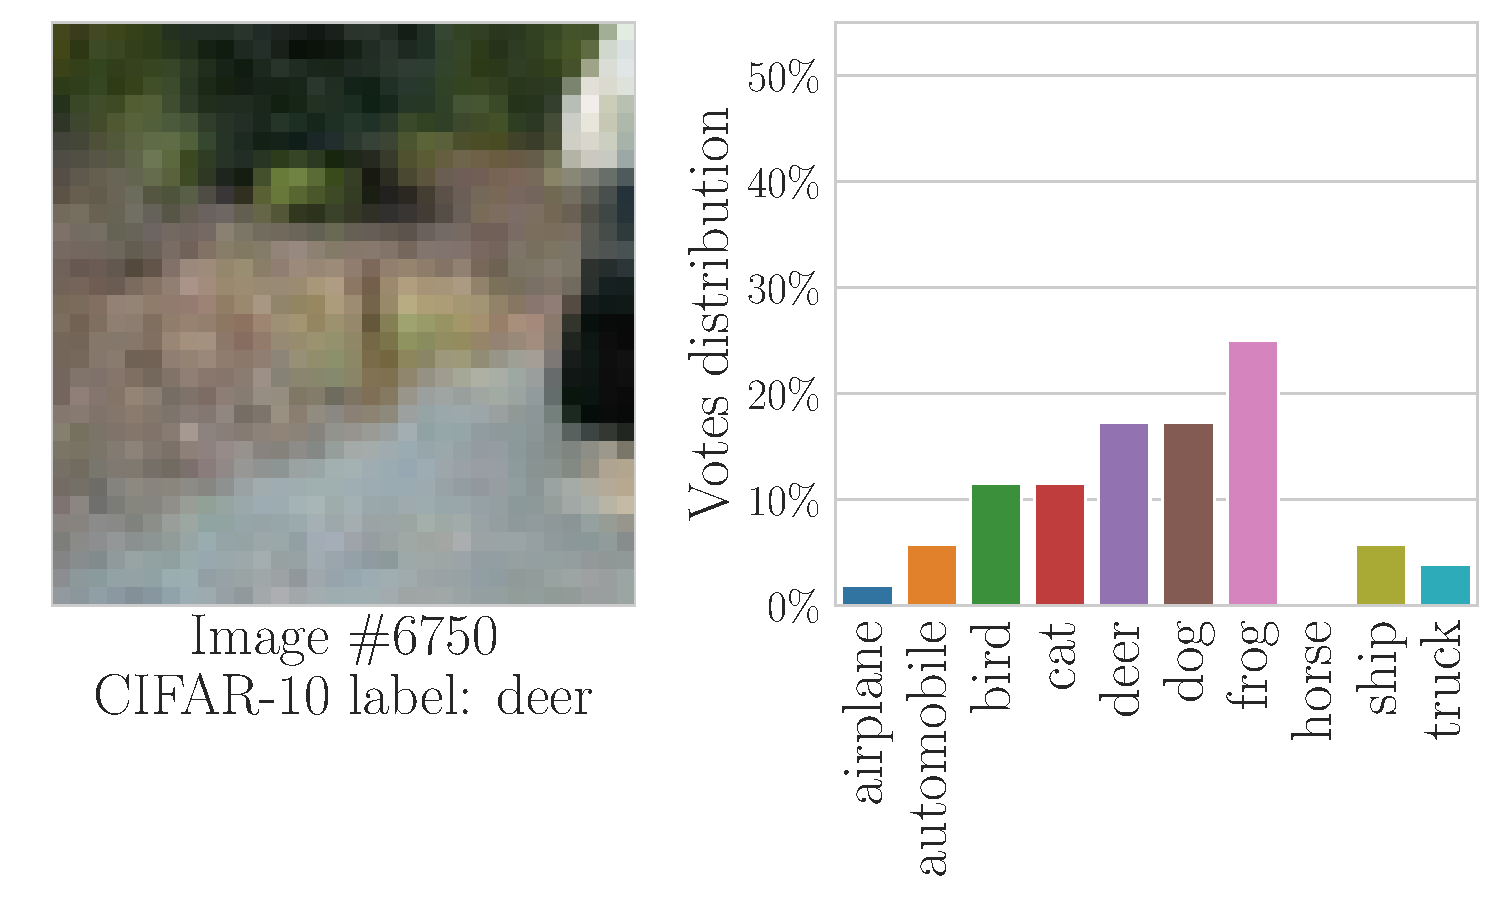
\includegraphics[width=\textwidth]{./chapters/images/image_n_hist6750_paper.pdf}}
    \end{minipage}%
    \hfill
    \begin{minipage}{.3\linewidth}
    \centering
    \subfloat[Label \texttt{airplane} is easy to identify (unanimity among workers).]{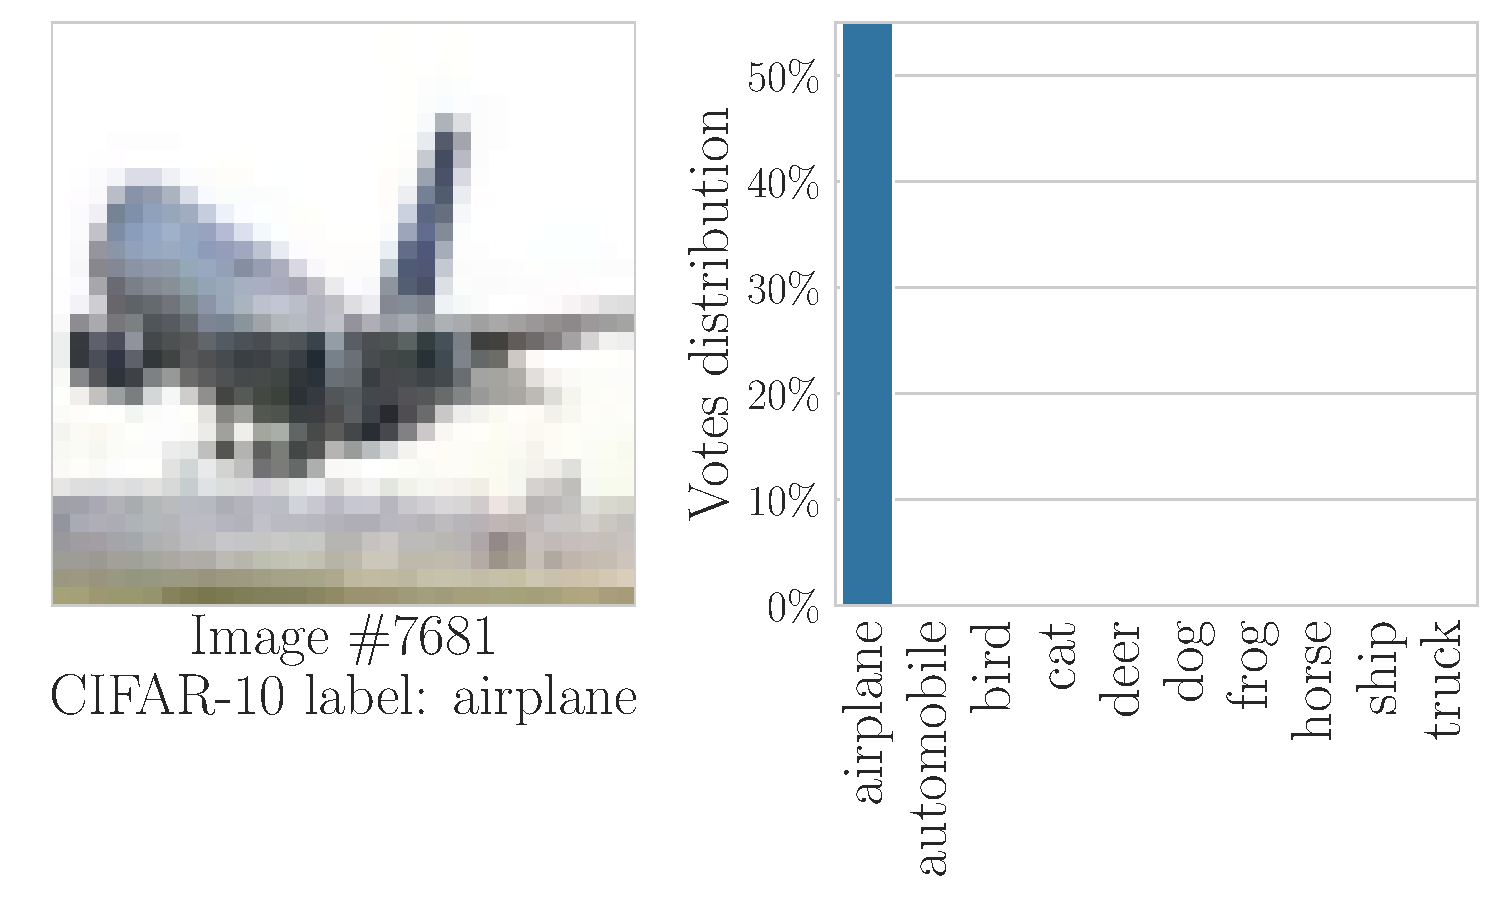
\includegraphics[width=\textwidth]{./chapters/images/image_n_hist7681_paper.pdf}}
    \end{minipage}%
    \hfill
    \begin{minipage}{.3\linewidth}
    \centering
    \subfloat[Label \texttt{cat} often confused with horns of a wild \texttt{deer}]{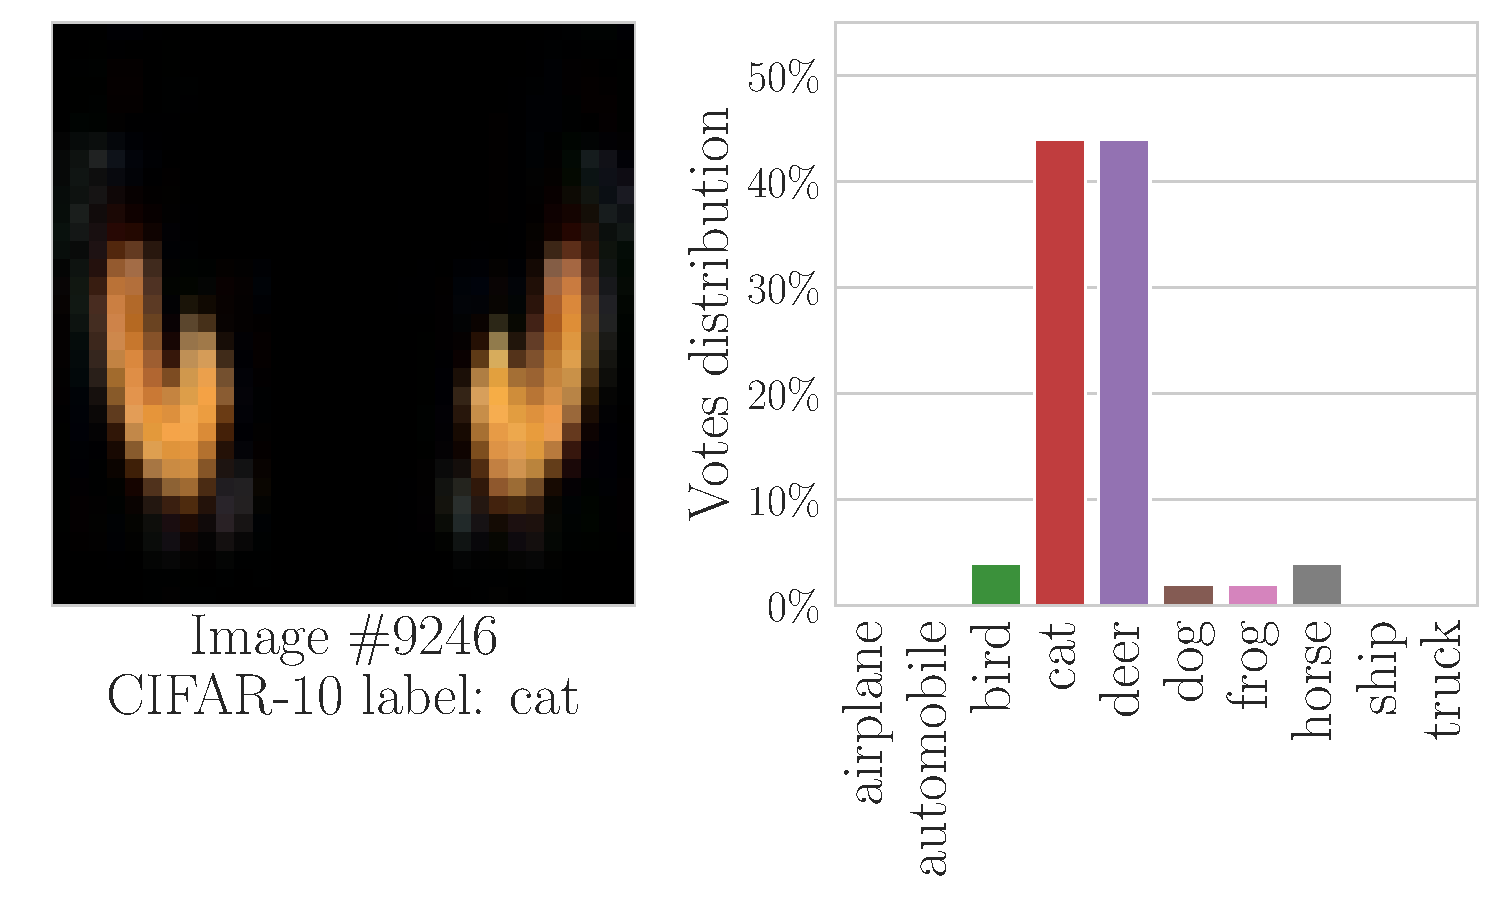
\includegraphics[width=\textwidth]{./chapters/images/image_n_hist9246_paper.pdf}}
    \end{minipage}
    \caption{Three images from \texttt{CIFAR-10H} dataset \citep{peterson_human_2019}, with the empirical distribution of workers' labels (soft labels): the \texttt{airplane} image (a) is easy, while the landscape (b) is ambiguous due to the image's poor quality. The last image (c) looks like a black cat face often perceived as the horns of a \texttt{deer}.}
    \label{fig:votes-c10h}
    \end{figure}

While the $\AUM$ shows results of identifying different types of sample difficulty by averaging the margin during $T>0$ training epochs, there is no direct way to apply it to the crowdsourcing setting.
Indeed, the $\AUM$ needs, by definition, a hard label $y_i$ to consider the assigned-label score $\mathcal{C}(x_i)_{y_i}$ and also to consider the second biggest score for a class different than $y_i$.
In the crowdsourcing setting however, there is no direct hard label $\hat y_i$ from the multiple answers $\{y_i^{(j)}\}_{j\in\mathcal{A}(x_i)}$ to a task $x_i$.


A naive transformation to apply the $\AUM$ in a crowdsourcing setting is to consider the majority voting aggregation. \Cref{eq:aum} simply becomes:
\begin{equation}\label{eq:aum_mv}
    \mathrm{AUMC}\left(x_i,\left\{y_i^{(j)}\right\}_{j\in\mathcal{A}(x_i)};\mathcal{D}_\texttt{train}\right) = \frac{1}{T}\sum_{t=1}^T \left[\sigma_{\hat y_i^{\mathrm{MV}}}^{(t)}(x_i) - \sigma_{[2]}^{(t)}(x_i)\right] \enspace.
\end{equation}
The $\AUM\mathrm{C}$ strategy lacks the worker abilities and task difficulty.
There is no worker-specific margin, the MV aggregation strategy removed the worker-specific information from the $\AUM$.
In the following, we introduce the $\WAUM$: a statistic that generalizes the $\AUM$ to the crowdsourcing setting by aggregating worker-specific margins into a weighted average to consider both worker abilities and task difficulty.

\subsection{Definition and construction of the WAUM}
% Explain weights choice and variations

We combine task difficulty scores with worker abilities scores, but we measure the task difficulty by incorporating feature information.
We thus introduce the Weighted Area Under the Margin ($\mathrm{WAUM}$), a generalization to the crowdsourcing setting of the Area Under the Margin ($\mathrm{AUM}$) by \citep{pleiss_identifying_2020}.
The $\mathrm{AUM}$ is a confidence indicator in an assigned label defined for each training task.
It is computed as an average of margins over scores obtained along the learning steps.
The $\mathrm{AUM}$ reflects how a learning procedure struggles to classify a task to an assigned label.
The $\mathrm{AUM}$ is well suited when training a neural network (where the steps are training epochs) or other iterative methods.
For instance, it has led to better network calibration \citep{park2022calibration} using MixUp strategy \citep{zhang2017mixup}, \emph{i.e.} mixing tasks identified as simple and difficult by the $\mathrm{AUM}$.
The $\mathrm{WAUM}$, our extension of the $\mathrm{AUM}$, aims at identifying ambiguous data points in crowdsourced datasets, so one can prune ambiguous tasks that degrade the generalization.
It is a weighted average of workers $\mathrm{AUM}$, where the weights reflect trust scores based on task difficulty and workers' ability.

Given several training epochs $T>0$ and a classifier $\mathcal{C}$ for a crowdsourced training set $\mathcal{D}_\text{train}$, we write the $\WAUM$ as a weighted average of worker specific $\AUM$.
Let $s^{(j)}(x_i)\in [0,1]$ be a trust factor in the answer of worker $w_j$ for task $x_i$.
The $\mathrm{WAUM}$ is then defined as:
\begin{align}
    \label{eq:WAUM}
    \mathrm{WAUM}(x_i)
     &
    = \tfrac{
    \displaystyle \sum_{j\in\mathcal{A}(x_i)}  \!\!\!
    s^{(j)}(x_i) \mathrm{AUM}\big(x_i, y_i^{(j)}\big)
    }
    {\displaystyle\sum_{j'\in\mathcal{A}(x_i)}
    s^{(j')}(x_i)}
    \enspace.
\end{align}
It is a weighted average of $\mathrm{AUM}$s over each worker's answer with a per task weighting score $s^{(j)}(x_i)$ based on workers' abilities.
This score considers the impact of the $\mathrm{AUM}$ for each answer since it is more informative if the $\mathrm{AUM}$ indicates uncertainty for an expert than for a non-expert.


The scores $s^{(j)}$ are obtained \emph{à la} \citet{servajean2017crowdsourcing}: each worker has an estimated confusion matrix $\hat{\pi}^{(j)}\in \mathbb{R}^{K\times K}$.
Note that the vector $\mathrm{diag}(\hat{\pi}^{(j)}) \in \mathbb{R}^{K}$ represents the probability for worker $w_j$ to answer correctly to each label.
With a neural network classifier, we estimate the probability for the input $x_i\in\mathcal{X}_\texttt{train} $ to belong in each category by $\smash{\sigma^{(T)}(x_i)}$, \emph{i.e.} the probability estimate at the last epoch.
As a trust factor, we propose the inner product between the diagonal of the confusion matrix and the softmax vector:
\begin{align}\label{eq:trust_factor}
    s^{(j)}(x_i) = \big\langle \mathrm{diag}(\hat{\pi}^{(j)}) , \sigma^{(T)}(x_i) \big\rangle \in [0,1] \enspace.
\end{align}
The scores control the weight of each worker in \Cref{eq:WAUM}.
This choice of weight is inspired by the bilinear scoring system of $\mathrm{GLAD}$ \citep{whitehill_whose_2009}, as detailed hereafter.
The closer to one, the more we trust the worker for the given task.
The score $s^{(j)}(x_i)$ can be seen as a multidimensional version of $\mathrm{GLAD}$'s trust score.
Indeed, in  $\mathrm{GLAD}$, the trust score is modeled as the product $\alpha_j\beta_i$, with $\alpha_j\in\mathbb{R}$ (resp. $\beta_i\in (0, +\infty)$) representing worker ability (resp. task difficulty).
In \Cref{eq:trust_factor}, the diagonal of the confusion matrix $\hat{\pi}^{(j)}$ represents the worker's ability and the softmax the task difficulty.


\paragraph{Why variance or entropy-based identifications are not always suited.}

The natural choice instead of the $\mathrm{WAUM}$ would be to use the entropy of the votes to detect ambiguous tasks. However, the entropy of the votes is not always suited for difficulty identification.
Indeed, when large amounts of votes per task are available, the entropy of the votes and the $\mathrm{WAUM}$ coincide well, as in \Cref{fig:entropy_vs_waum}(a).
Yet, when votes are scarce, as in \Cref{fig:entropy_vs_waum}(b) and (c), entropy becomes irrelevant while our introduced $\mathrm{WAUM}$ remains useful.

\begin{figure}[thb]
    \centering
    \hfill
    \subfloat[\texttt{CIFAR-10H} dataset.]{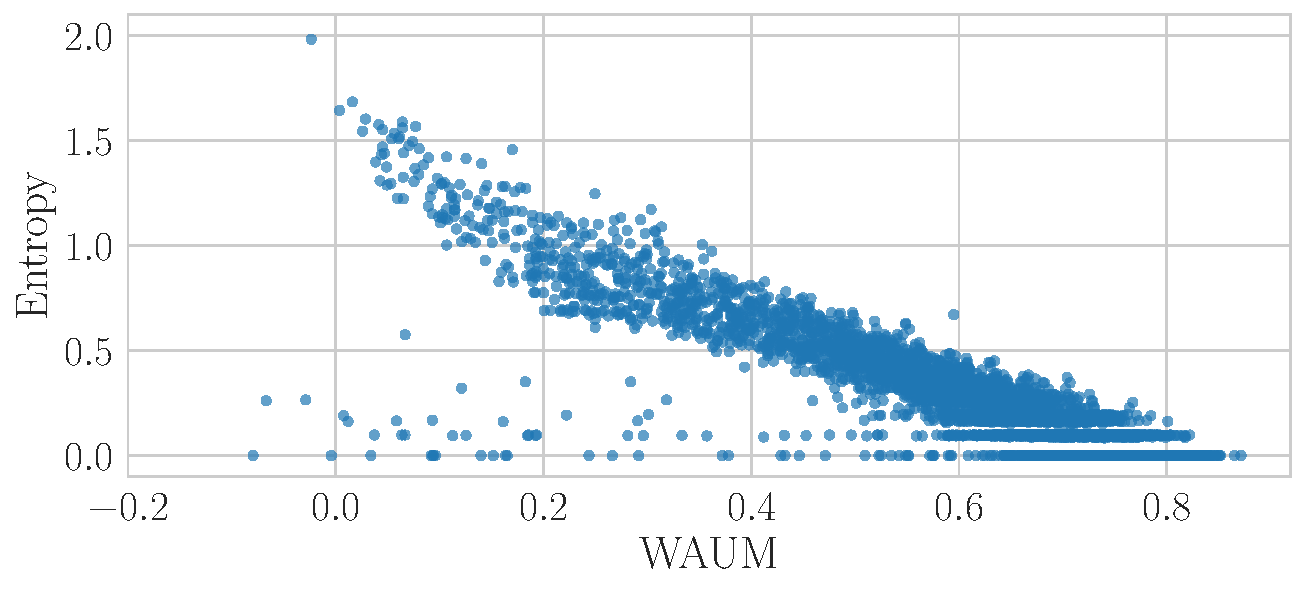
\includegraphics[width=0.3083\textwidth]{images/scatter_entropy_vs_waum_CIFAR-10H.pdf}}
    \hfill
    \subfloat[\texttt{LabelMe} dataset.]{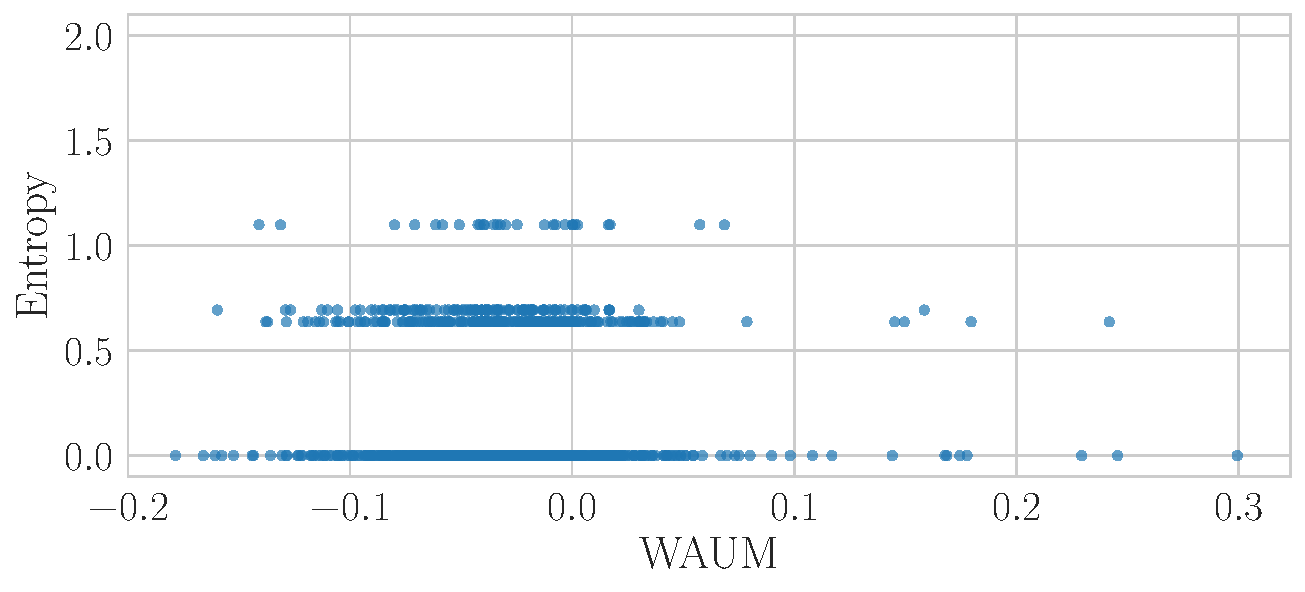
\includegraphics[width=0.3083\textwidth]{images/scatter_entropy_vs_waum_LabelMe}}
    \hfill
    \subfloat[\texttt{Music} dataset.]{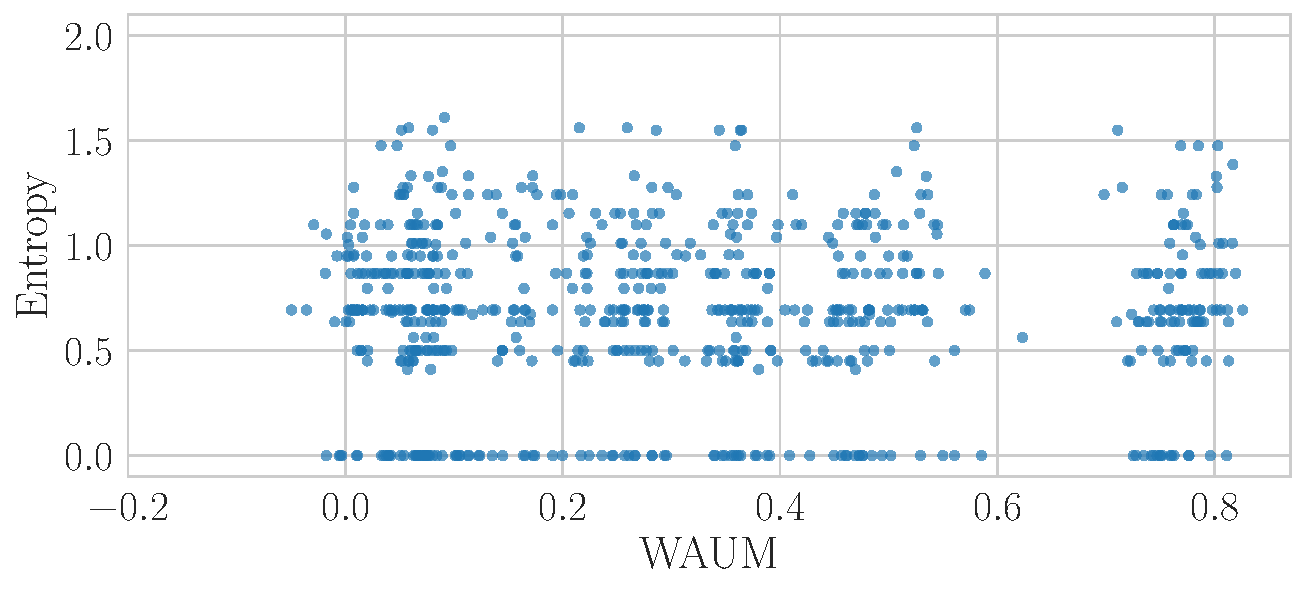
\includegraphics[width=0.3083\textwidth]{images/scatter_entropy_vs_waum_Music}}
    \hfill
    \caption{Entropy of votes vs. $\mathrm{WAUM}$ for \texttt{CIFAR-10H}, \texttt{LabelMe}, and \texttt{Music}, each point representing a task/image. When large amounts of votes per task are available, $\mathrm{WAUM}$ and entropy ranking coincide well, as in (a). Yet, when votes are scarce, as in (b) and (c), entropy becomes irrelevant while our introduced $\mathrm{WAUM}$ remains useful. Indeed, tasks with few votes can benefit from feedback obtained for a similar one. And for the \texttt{LabelMe} dataset in particular, there are only up to three votes available per task, thus only four different values of the entropy possible, making it irrelevant in such cases for modeling task difficulty.}
    \label{fig:entropy_vs_waum}%
\end{figure}

\paragraph{Dataset Pruning.} Our procedure (\Cref{alg:WAUMstack}) proceeds as follows.
We initialize our method by estimating the confusion matrices for all workers.
For each worker $w_j$, the $\mathrm{AUM}$ is computed for its labeled tasks, and so is its worker-dependent trust scores $s^{(j)}(x_i)$ with \Cref{eq:trust_factor} during the training phase of a classifier.
The $\mathrm{WAUM}$ in \Cref{eq:WAUM} is then computed for each task.
The most ambiguous tasks, the ones whose $\mathrm{WAUM}$ are below a threshold, are then discarded, and the associated pruned dataset $\mathcal{D}_{\text{pruned}}$ is output. We consider for the pruning threshold a quantile of order $\alpha\in[0,1]$ of the $\mathrm{WAUM}$ scores.
The hyperparameter $\alpha$ (proportion of training data points pruned) can be chosen on a validation set, yet choosing $\alpha\in\{0.1, 0.05, 0.01\}$ has led to satisfactory results in all our experiments.
Note that the same pruning procedure can be applied to $\mathrm{AUMC}$ for comparison.
Both the $\mathrm{AUMC}$ and $\mathrm{WAUM}$ inherit the hyperparameter $T>0$ from the original $\mathrm{AUM}$.
Following the recommendations from \citet{pleiss_identifying_2020}, we need $T$ large enough for stability and $T$ not too big to avoid overfitting the data.
In practice, a guideline given is to train until the first learning rate scheduler drops to only keep the beginning of the scores trajectories without finetuning.
The main assumptions to identify ambiguous tasks is thus not to over-train the neural network in the $\mathrm{WAUM}$ (or $\mathrm{AUMC}$) step, and to be able to run a DS-like algorithm to recover the diagonal of the confusion matrix for \Cref{eq:trust_factor}.

\paragraph*{Refined initialization: estimating confusion matrices.}
By default, we rely on the \texttt{Est}$=$DS algorithm to get workers' confusion matrices, but other estimates are possible: DS might suffer from the curse of dimensionality when the number $K$ of classes is large ($K^2$ coefficients needed per worker).

\begin{algorithm}[tb]
\caption{$\mathrm{WAUM}$ (Weighted Area Under the Margin).}
\label{alg:WAUMstack}
\textbf{Input}:  $\mathcal{D}_{\texttt{train}}$: tasks and crowdsourced labels, $\alpha\in[0,1]$: proportion of training points pruned, $T\in \mathbb{N}$: number of epochs, $\texttt{Est}$: Estimation procedure for the confusion matrices\\
\textbf{Output}: pruned dataset $\mathcal{D}_{\text{pruned}}$
\begin{algorithmic}[1]
\STATE Get confusion matrix $\{\hat{\pi}^{(j)}\}_{j\in[n_\texttt{worker}]}$ from \texttt{Est}
\STATE Train a classifier for $T$ epochs on $\left(x_i, y_i^{(j)}\right)_{i,j}$
\FOR{$j\in[n_\textrm{worker}]$}
\STATE Get $\mathrm{AUM}(x_i, y_i^{(j)}; \mathcal{D}_{\texttt{train}})$ using \Cref{eq:Margin_WAUM} for $i\in\mathcal{T}(w_j)$
\STATE Get \textbf{trust scores} $s^{(j)}(x_i)$ using \Cref{eq:trust_factor} for $i\in\mathcal{T}(w_j)$
\ENDFOR
\FOR{each task $x\in\mathcal{X}_\texttt{train}$}
\STATE Compute $\mathrm{WAUM}(x)$ using \Cref{eq:WAUM}\;
\ENDFOR
\STATE  Get $q_{\alpha}$ $(\mathrm{WAUM}(x_i))_{i\in[n_\texttt{task}]}$, $\alpha$-\textbf{quantile threshold}
\STATE $\mathcal{D}_{\text{pruned}}\!=\!
        \Big\{
        \big( x_i, \big(y_i^{(j)}\big)_{j\in\mathcal{A}(x_i)}\big) \! : \!\mathrm{WAUM}(x_i) \geq q_\alpha,  x_i \in \mathcal{X}_\texttt{train}  \Big
        \}$
\end{algorithmic}
\end{algorithm}

%%%%%%%%%%%%%%%%%%%%%%%%%%%%%%%%%%%%%%%%%%%%%%%%%%%%%%%%%%%%%%%%%%%%%%%%%%%%%%%
\paragraph{Training on the pruned dataset}
%%%%%%%%%%%%%%%%%%%%%%%%%%%%%%%%%%%%%%%%%%%%%%%%%%%%%%%%%%%%%%%%%%%%%%%%%%%%%%%
Once a pruned dataset $\mathcal{D}_{\text{pruned}}$ has been obtained thanks to the $\mathrm{WAUM}$, one can create soft labels through an aggregation step, and use them to train a classifier.
Aggregated soft labels contain information regarding human uncertainty, and could often be less noisy than NS labels.
They can help improve model calibration \citep{wen2020combining, zhong2021improving}, a property useful for interpretation \citep{jiang2012calibrating, kumar2019verified}.
Concerning the classifier training, note that it can differ from the one used to compute the $\mathrm{WAUM}$.
We train a neural network whose architecture is adapted dataset per dataset and that can differ from the one used in \Cref{alg:WAUMstack} (it is the case for instance for the \texttt{LabelMe} dataset).
For an aggregation technique $\texttt{agg}$, we write the full training method on the pruned dataset created from the $\mathrm{WAUM}$: $\texttt{agg}+\mathrm{WAUM}$ and instantiate several choices in our experiments.
For comparison, we write $\texttt{agg} + \mathrm{AUMC}$ the training method on the pruned dataset created from the $\mathrm{AUMC}$.


\subsection{Evaluating the WAUM}


\subsection{Results on simulated datasets}
Circles (good) + Two moons (not all ambiguities are to be removed)

\subsection{Results on datasets with tasks available}
CIFAR-10H + LabelMe + Music

\subsection{Where can these errors come from? Going back to the dataset creation and discussion}
(motivation + transition for the need of WAUM)
Example of CIFAR-10 to CIFAR-10H. The lack of explainations in crowdsourcing. Recent conference (Neurips) ask for detailed explainations now for new datasets, but crowdsourced data is often not released.
